% 美赛模板:正文部分

\documentclass[12pt]{article}  % 官方要求字号不小于 12 号,此处选择 12 号字体
% \linespread{1.1}
% \bibliographystyle{plain}
% 本模板不需要填写年份,以当前电脑时间自动生成
% 请在以下的方括号中填写队伍控制号
\usepackage[2406905]{easymcm}  % 载入 EasyMCM 模板文件
\problem{C}  % 请在此处填写题号
\usepackage{mathptmx}  % 这是 Times 字体,中规中矩 
% \usepackage{palatino}  % mathpazo 这palatino是 COMAP 官方杂志采用的更好看的 Palatino 字体,可替代以上的 mathptmx 宏包
\usepackage{pdfpages}
\usepackage{longtable}
\usepackage{tabu}
\usepackage{threeparttable}
\usepackage{listings}
\usepackage{paralist}
\usepackage{placeins}  % 避免图片乱跑,要在图片后面加上\FloatBarrier
\usepackage{wallpaper} % 海报页背景
\usepackage{enumitem}
\usepackage{setspace}
% AI report
\usepackage{ulem} % 引入 ulem 包以支持下划线
\usepackage[most]{tcolorbox} % 引入 tcolorbox 包
\usepackage{xcolor} % 引入 xcolor 包

 \let\itemize\compactitem
 \let\enditemize\endcompactitem
\newcommand{\upcite}[1]{\textsuperscript{\textsuperscript{\cite{#1}}}}
\title{Momentum: The Ethereal Arsenal Above the Skies, \\Guiding Triumph}  % 标题

% 如需要修改题头(默认为 MCM/ICM),请使用以下命令(此处修改为 MCM)
%\renewcommand{\contest}{MCM}

% 文档开始
\begin{document}

% 此处填写摘要内容
\begin{abstract}
    

    
In tennis, a player's performance can fluctuate over multiple points or even games, and the player with the upper hand in power may not be able to win. The aim of this paper is to create a momentum-centred system that explores the relationship between momentum and the match, and provides accurate dynamic predictions of match situations.

For the first part, we built a \textbf{momentum index model} based on the \textbf{G1-Entropy -Independ-}\textbf{ence} Weight integrated evaluation method. With this integrated evaluation method, we identified different weights for different data. Subsequently, we calculated the momentum indices of the players before the start of the match to assess the quality of their performance and the degree of their dominance. Next, we qualitatively compared the momentum indices with score point curve and game point curve to visualise trends in tennis matches.

For the second part, we establish a matching system between the momentum index and player performance based on \textbf{DTW}. We represent continuous scores in terms of continuous highlight performances. Subsequently, we match the player momentum index curve, the point score curve and the games score curve by the dynamic time regularisation algorithm to get the match between the momentum index curve and the two curves. Eventually, it was found that the matching degree of momentum index curve with point score curve and games score curve reached 88.635\% and 91.156\%, respectively. This suggests that momentum plays a key role in games and that the coach's claim is either incorrect or not rigorous.

For the third part, we applied the \textbf{LSTM} model in deep learning and compared it with the \textbf{ARIMA} prediction model, and found that the LSTM model is more accurate and better. At the same time, we applied the LSTM model for prediction, and the accuracy of the validation set reached 81.32\%, and the loss rate was reduced to 0.07, which is already a very high accuracy. Not only that, we also gave constructive advice to the athletes on how to prepare for the game when facing new opponents from the three dimensions of opponent, player's self, and on-site factors.

For the fourth part, we chose data from the 2023 NBA Eastern Conference Finals game between the Heat and the Celtics. We included pre-game player psychological pressure, the course of the first six games as considerations in the momentum index model developed. We then matched the momentum index curve to the scoring uptick curve of the game and found a match rate of 65.918\%. Based on the momentum index model, we conclude that the Heat will win, which also matches the final result.

Finally, we provided a non-technical report and conducted \textbf{sensitivity analysis} of the evaluation model, demonstrating the robustness and accuracy of the model.

    \vspace{5pt}
    \textbf{Keywords}: G1-Entropy-Independence \hspace{5pt}  DTW \hspace{5pt} ARIMA \hspace{5pt} LSTM  \hspace{5pt}

\end{abstract}

\maketitle  % 生成 Summary Sheet

\tableofcontents  % 生成目录


\section{Introduction}
\subsection{Problem background}

In the 2023 Wimbledon final, 36-year-old Novak Djokovic lost for the first time at Wimbledon since 2013 when he was defeated 2:3 by 20-year-old Alcaraz. In the first set, Djokovic crushed to a 6:1 win. But Alcaraz came out of nowhere to win 3:2 in the following game. It was a landmark match, no doubt about it. But at the same time, there was a lot of discussion about how Alcaraz was able to regain his confidence and win the match after losing the first set. One element that was brought up was the player's momentum, which is affected by all aspects of the player's game, but can be countered by the player's new game, and whose magnitude is a key factor in whether or not the player is able to win.

\subsection{Restatement of the Problem}

Consider the background information, we need to complete the following tasks in sequence:

\begin{itemize}
    \item Build a momentum index model to determine which player is performing better at a given moment and visualize the changing game situation.
    \item Establish the matching system of momentum and victory, evaluate the coach's opinion, and make a quantitative evaluation of whether the momentum is real.
    \item Build a match trend prediction model based on players' form to identify turning points in matches and give players advice on how to prepare for matches.
    \item We need to transfer the momentum index model of tennis matches to other matches to see if the model is still valid and whether the model is widely used.
\end{itemize}

\subsection{Literature Review}

This subject focuses on simulating player momentum and investigating the flow of events throughout a tennis match. After doing a thorough literature search, our team discovered the following three main strategies:

\begin{itemize}
    \item First, deep learning with neural networks[1] and machine learning-based modeling using popular techniques like logistic regression[2], random forests[3], and so on.
    \item Another strategy that uses extensive simulations instead of computing methods is Monte Carlo-based simulations[4].
    \item In the end, it is based on the methods of evaluation, and we discovered G1[5], the independence weight method[6], the entropy weight method[7], etc.
\end{itemize}

The specific method is shown below:

\begin{figure}[h] % 开始一个浮动体环境,[h]指定为 here(这里)位置
	\centering % 图片居中
	\includegraphics[width=0.73\textwidth]{picture/文献综述.pdf} % 插入宽度为文本宽度一半的图片
	\caption{Literature Review Framework} % 图片标题
	\label{} % 图片标签,用于引用
\end{figure}
\FloatBarrier

After considering many trade-offs, our team decided to integrate deep learning modeling with evaluation techniques.

\subsection{Our work}

The entire modeling process is as follows:

\begin{figure}[h] % 开始一个浮动体环境,[h]指定为 here(这里)位置
	\centering % 图片居中
	\includegraphics[width=0.7\textwidth]{picture/our_work.pdf} % 插入宽度为文本宽度一半的图片
	\caption{Model framework} % 图片标题
	\label{} % 图片标签,用于引用
\end{figure}
\FloatBarrier

\section{Assumptions and Justifications}
The following basic assumptions are made to simplify problems.
      
    \textbf{Assumption 1:} We assume that external factors such as weather, spectators, etc. do not affect the player's performance, so that the model and its results are fully analysed from the available data.
    
    \textbf{Justification 1:} In fact players' play can be affected by factors such as wind speed, sunlight, and whether or not the spectators are disciplined in the game, and disregarding these can help us simplify the model.
    
    \textbf{Assumption2:} We assume that the players are all in the same physical condition before starting the match.
    
    \textbf{Justification 2:} Wimbledon is a knockout format, and player fitness is theoretically affected by the previous matches, but since we don't know a player's fitness reserves or original fitness status, it is assumed that the two players before the match were in the same physical condition.
    
    \textbf{Assumption 3:} We assume that players' psychological factors are not affected by their record against their opponents.

    \textbf{Justification 3:} In actual matches, players' psychology and strategy will be affected by past performance, which is too difficult to be considered due to the statistics.

    
    \newpage

\section{Notations}
The primary notations used in this paper are listed in Table \ref{tab:notation}.

\begin{table}[htbp]
    \centering
    \caption{Notations}
    \label{tab:notation}
    \begin{tabular}{m{4cm}<{\centering}m{10cm}<{\centering}}
    \toprule[2pt]
    Symbol & Description \\
    \midrule[1pt]
    $n$ & Number of data points \\[0.5ex]
    $(x_{i},y_{i})$ & Represents the coordinates of the i-th data point \\[0.5ex]
    $x_{i}^{'}$ & The i-th data point after minimum maximum normalization \\[0.5ex]
    $x_{\max}$ & Maximum value in the original dataset \\[0.5ex]
    $x_{\min}$ & The minimum value in the original dataset \\[0.5ex]
    $b_{i}$ & Indicator set \\[0.5ex]
    $r_{j}^{a}$ & The a-th person judges the weight ratio between adjacent indicators $b_{j}$ and $b_{f}$ \\[0.5ex]
    $w_{n}$ & The final weight of indicator $b_{n}$ \\[0.5ex]
    $B$ & Non negative standard matrix \\[0.5ex]
    $H_{j}$ & The entropy value of the j-th evaluation indicator $b_{j}$ \\[0.5ex]
    $p_{ij}$ & The proportion of data for the i-th time under the j-th indicator \\[0.5ex]
    $W_{j}$ & The comprehensive weight vector of all indicators \\[0.5ex]
    $x_{i}$ & Represent whether i scored at a specific time point \\[0.5ex]
    $y_{i}$ & Momentum index at time point i \\[0.5ex]
    $D$ & Cost matrix \\[0.5ex]
    $S$ & Matching score \\[0.5ex]
    $M_{i}$ & Player i's momentum \\[0.5ex]
    $P_{i}$ & Player i's winning rate \\[0.5ex]
    $f_{t}$ & Forgetting Gate \\[0.5ex]
    $i_{t}$ & input Gate \\[0.5ex]
    $c_{t}$ & Control the candidate state at the current moment \\[0.5ex]
    $o_{t}$ & Output gate \\[0.5ex]
    \bottomrule[2.5pt]
    \end{tabular}
\end{table}
    

\section{Model I: The Momentum Index Model for the Match Flow}

\subsection{Indicator Integration and Information Synthesis}
We believe that momentum can help us capture the flow of the game during a match, so building a model that captures the flow is equivalent to building a momentum index model.

As momentum is related to various conditions and data during the game, we categorized and summarized the data for each set of variables detected during the game. It was classified into five dimensions: course of the match, match pressure, offensive ability, physical condition and defensive ability. Each dimension is characterized by two to nine specific indicator variables, and the structural relationship between each dimension and its internal indicators is shown in Figure \ref{fig:m1_work}:

\begin{figure}[h] % 开始一个浮动体环境,[h]指定为 here(这里)位置
	\centering % 图片居中
	\includegraphics[width=0.85\textwidth]{picture/第一问的指标.pdf} % 插入宽度为文本宽度一半的图片
	\caption{Classification chart of indicator information} % 图片标题
	\label{fig:m1_work} % 图片标签,用于引用
\end{figure}
\FloatBarrier

\subsection{The G1-Entropy-Independence Weight Comprehensive Evaluation\\ Method}
The weights of different types of indicators can reflect the amount of information of different levels of importance contained in different types of indicators. However, due to the wide variety of assessment indicators, there is inevitably information redundancy between indicators. Therefore, this paper proposes a comprehensive assessment method called G1-Entropy-Independence Weight (G1-Entropy-Independence Weight).

The method calculates the composite weight of each momentum indicator of the athlete by combining subjective weighting methods (ordinal analysis method (G1 method)) with objective weighting methods (entropy weighting and independent weighting methods). A certain amount of human subjectivity can be mitigated and changes in objective situations can be reflected by combining subjective and objective weighting techniques. The use of the independent weights method can improve the problem of over-sensitivity in the entropy weights method, reduce the problem of redundant information between indicators, and supplement the subjective weight determination method to finally assess the athlete's condition.

The process flow of this method is as follows:

\begin{figure}[h] % 开始一个浮动体环境,[h]指定为 here(这里)位置
	\centering % 图片居中
	\includegraphics[width=0.7\textwidth]{picture/第一问的流程图.pdf} % 插入宽度为文本宽度一半的图片
	\caption{Evaluation method flowchart} % 图片标题
	\label{fig:example} % 图片标签,用于引用
\end{figure}
\FloatBarrier

\subsubsection{Data Preprocessing}

\noindent\textbf{Linear Fit Filling}

Missing values may lead to biases in the dataset that may mislead the final conclusions, such as missing values in ball speed. Therefore, it is necessary to perform a linear fit to the attribute columns with missing values to fill them. The mathematical principle used in linear fitting is the method of least squares[8], which requires finding a line that minimises the sum of the distances from all data points to the line, i.e. solving the following equation:

\begin{eqnarray}
	\mathop{min}_{a, b} \sum_{i=1}^n(y_i-(ax_i+b))^2
\end{eqnarray}

where \(n\) is the number of data points and \((x_i, y_i)\) represents the coordinates of the \(i\) th data point. The method involves summing the error squares of the \(n\) data points, i.e., the sum of the squares of the distances from each data point to the fitted line. The least squares approach aims to minimize this sum of squares by determining the values of \(a\) and \(b\).

\noindent\textbf{Min-Max Normalization}

Throughout the Excel dataset, there are a number of tennis-related metrics, such as depth, ball speed, and so on. Different metrics have different units and dimensions, and their value ranges, sizes and units vary significantly. This may lead to bias and errors in the results of data analysis. In order to eliminate the influence of dimensions and value ranges between data metrics on the results and to make different metrics comparable and analyzable[9], we scaled the raw data to the range [0,1] using min-max normalization. This process ensures that each indicator is comparable. The formula for normalization is given below:

\begin{eqnarray}
	x_i'=x_{min}+\dfrac{x_j-x_{min}}{x_{max}-x_{min}}
\end{eqnarray}

where \(x_i'\) is the \(i^{th}\) data point after min-max normalization, and \(x_{max}\) and \(x_{min}\) are the maximum and minimum values in the original dataset, respectively.

\subsubsection{Utilizing the G1 Method to Determine Subjective Weights}

The advantage of the G1 method[10] over hierarchical analysis is that it does not require consistency checks. In addition, it can overcome inaccuracies due to the hesitation of experts in making judgements when many indicators are present. It can establish the subjective weights rapidly and precisely, giving experts assessments a solid platform.

For each set of indicators \( b_1, b_2, \cdots, b_n \), the specific steps for using the G1 weighting method are as follows:

\begin{table}[H]
	\centering
	\caption{The G1 Weighting Method for Indicator Sets}
	\label{my-label}
	\begin{tabular}{@{}p{0.95\textwidth}@{}}
	\toprule
	\textbf{Algorithm 1: The G1 Weighting Method for Indicator Sets} \\ \midrule
	\textbf{Input:} Indicator set \( \{b_1, b_2, \ldots, b_n\} \), number of indicators \( n \), number of experts \( p \), weight ratio values \( \{1.0, 1.2, 1.4, 1.6, 1.8\} \) \\
	\textbf{Step 1:} For each expert \( a \), identify the least important indicator \( b_n \), then the second least important \( b_{n-1} \), and so on, until a unique ordering is obtained. \\
	\textbf{Step 2:} Calculate the weight of the least important indicator \( w_n^a \) using Equation (3): 
	% \[ w_n^a = \frac{1}{1 + \sum_{k=1}^{n-1}\prod_{j=k}^{n-1}(r_j^a - 1)} \] \\
    \begin{equation}
        w_n^a = \frac{1}{1 + \sum_{k=1}^{n-1}\prod_{j=k}^{n-1}(r_j^a - 1)}
    \end{equation}
	\textbf{Step 3:} Calculate the weights of other indicators using the recursive formula (4): 
	% \[ w_{k-1}^a = \frac{w_k^a}{r_{k-1}^a} \] \\
    \begin{equation}
        w_{k-1}^a = \frac{w_k^a}{r_{k-1}^a}
    \end{equation}
	\textbf{Step 4:} Average the weights of the \( n^{th} \) indicator obtained from all experts to calculate the final weight \( w_n \) using Equation (5): 
	% \[ w_n = \frac{\sum_{a=1}^{p}w_n^a}{p} \] \\
    \begin{equation}
        w_n = \frac{\sum_{a=1}^{p}w_n^a}{p}
    \end{equation}
	\textbf{Output:} Final weight for each indicator \( \{w_n\} \). \\ \bottomrule
	\end{tabular}
\end{table}

\subsubsection{Determining Objective Weights Using the Entropy Weight Method}

An objective way for determining the weights of different indicators based on the quantity of information they carry is the entropy weighting method[11]. An indicator of the quantity of information is entropy. An indicator's entropy decreases with more information and variability in a complex decision-making scenario. Therefore, the more weight the indicator has, the more important it is in weighing possibilities[12]. This approach minimizes the impact of subjective opinions and has straightforward computation procedures, increased impartiality, and efficient data utilization.

Since the original data matrix has been processed into a dimensionless, non-negative standard matrix \(B = (b_{ij})_{m \times n}\):

\begin{equation}
	\boldsymbol{B} =
	\begin{bmatrix}
		b_{11} & b_{12} & \cdots & b_{1n}\\
		b_{21} & b_{22} & \cdots & b_{2p}\\
		\vdots & \vdots & \ddots & \vdots\\
		b_{m1} & b_{m2} & \cdots & b_{mn}\\
	\end{bmatrix}
\end{equation}

In the evaluation of an athlete's momentum over \(m\) time points and \(n\) evaluation indicators, the entropy value of the \(j^{th}\) evaluation indicator \(b_j\) is defined as:

\begin{equation}
	H_j=-K\sum_{i=1}^m p_{ij}\ln p_{ij}, \quad j=1,2,\ldots,n
\end{equation}

Where

\begin{equation}
	\begin{cases}
		K=\frac{1}{\ln m}\\[8pt]
		p_{ij}=\dfrac{b_{ij}}{\sum_{i=1}^mb_{ij}}
	\end{cases}
\end{equation}

In the formula, \(p_{ij}\) is the proportion of the data at time \(i\) for indicator \(j\). It is also stipulated that: when \(p_{ij} = 0\), \(p_{ij} \ln p_{ij} = 0\).

Then, the entropy weight of the \(j^{th}\) indicator is defined as:

\begin{equation}
	w'_j=\frac{1-H_j}{\sum_{j=1}^n(1-H_j)}
\end{equation}

\subsubsection{Determining Objective Weights Using the Independence Weight Method}

While the entropy weighting method can effectively use data to minimize the impact of subjective expert opinion, it determines weights based solely on the amount of information contained in each individual indicator, without taking into account the overlap of information between indicators. If these indicators are used directly for assessment, information redundancy may occur, thus reducing the accuracy of the assessment[13]. Therefore, this paper adopts the independent weight method to consider the interrelationship between indicators. Combined with the entropy weight method, a composite objective weight of the indicators is formed, making the assessment results more accurate.

The independent weight coefficient method determines weights by calculating the coefficient of partial correlation between indicators[14]. The degree of redundant correlation can be assessed by calculating the partial correlation coefficient, which is a measure of the correlation between a dependent variable and a group of independent variables. The higher the partial correlation coefficient, the more redundant the information and the lower the weight. Using the inverse of the partial correlation coefficient as the weighting factor reflects the amount of information in the assessment indicators that is significantly different from the other indicators, effectively addressing the issue of redundant information between indicators.

In assessing the momentum of athletes, each group of indicators contains \(\{b_1, b_2, \ldots, b_n\}\). If the indicator \(b_1\) has a stronger linear relationship with the other indicators, this means that \(b_1\) can be represented by a linear combination of the other indicators; from another point of view, this means that there is more redundant information, and therefore the weight of this indicator should be smaller. The formula for calculating the partial correlation coefficient \(R_j\) of the indicator \(b_j\) is as follows:

\begin{equation}
	R_j=\frac{\sum_{j=1}^n (b_j-\bar{b})(\tilde{b}-\bar{b})}{\sqrt{\sum_{j=1}^n(b_j-\bar{b})^2\sum_{j=1}^n(\tilde{b}-\bar{b})^2}}
\end{equation}

In the formula, \(\tilde{b}\) is the matrix obtained from matrix \(B\) by removing the column corresponding to \(b_j\); \(\bar{b}\) is the average value of the matrix \(B\).

Since there is an inverse relationship between \(R_j\) and the weight \(w''_j\), by selecting the reciprocal of \(R_j\) and then normalizing it, the weight values for each indicator can be determined. The final formula for calculating the weights is:

\begin{equation}
	\begin{cases}
		R=\left(\frac{1}{R_1},\frac{1}{R_2},\ldots,\frac{1}{R_n}\right) \\[8pt]
		w''_j=\dfrac{\frac{1}{R_j}}{\sum_{j=1}^nR_j}
	\end{cases}
\end{equation}

\subsubsection{Determination of Composite Weights}
After determining the weights \(w \bar{_j}\), \(w'_j\), and \(w''_j\) using the G1 method, the independence weight coefficient method and the entropy weight method, respectively, the composite weight for the \(j^{th}\) indicator can be obtained using the product method in the combination of weights as:

\begin{equation}
	w_j=\frac{\bar{w}_jw'_jw''_j}{\sum_{j=1}^n\bar{w}_jw'_jw''_j}
\end{equation}

Then the composite weight vector \(W_j\) for all indicators is:

\begin{equation}
	W_j=[w_1,w_2,\ldots,w_n]^T
\end{equation}

\subsubsection{Determination of the Momentum Formula}

At this point, the momentum formula can be determined as follows:

\begin{equation}
	P = \sum_{i=1}^n w_i x_i
\end{equation}

After incorporating the match data of Djokovic and Alcaraz, we have drawn a chart showing the momentum trend changes of the two players:

\begin{figure}[h] % 开始一个浮动体环境,[h]指定为 here(这里)位置
	\centering % 图片居中
	\includegraphics[width=0.7\textwidth]{picture/momentum_adjustment_no_title.pdf} % 插入宽度为文本宽度一半的图片
	\caption{Trend chart of player momentum indicators} % 图片标题
	\label{fig:example} % 图片标签,用于引用
	\end{figure}
\FloatBarrier

Not only that, we also drew the scoring curves of the players and the point scoring curves of the games, facilitating a comprehensive assessment of the flow of the game situation:

\begin{figure}[htbp]
    \centering    
    \subfigure[]{				% 图片1([]内为子图标题)
    \label{Fig.sub.Flexibility_33.70}							% 子图1的标签
    \includegraphics[width=0.45\textwidth]{picture/折线图1.pdf}}			  % 子图1的相对位置
    \subfigure[]{				% 图片2
    \label{Fig.sub.Flexibility_26.66}						% 子图2的标签
    \includegraphics[width=0.45\textwidth]{picture/折线图.pdf}}
    \caption{Trend chart of player point score and game score}		% 总图标题
    \label{Fig:Flexibility}									% 总图标签
\end{figure}

The momentum trend chart shows that Djokovic took the lead at the start of the match and won the first set. In fact, Alcaraz chose to strategically give up some sets when he was clearly behind in the game. In this way, Alcaraz ended up winning the match by virtue of his leading disc score, despite scoring lower in the total number of discs. The momentum trend graph also shows the specific performances of both players - although Alcaraz lost some games and points, he did so strategically and did not affect his momentum. Despite fluctuating momentum and alternating leads during the match, Alcaraz still performed better.

\section{Model II:Momentum-Performance Matching System Based on DTW}
In problem 2, a coach questions the existence of the "momentum" factor, arguing that players' performance fluctuations and scoring streaks are random. We need to develop an index and create a calculation system to evaluate coaches' statements about the randomness of players' performance fluctuations and scoring streaks, and to explore the relationship between the momentum index and players' wins and losses, as well as their scoring streaks.

For this purpose, we use the Dynamic Time Warping (DTW) algorithm[15] to build a DTW-based matching system between momentum indices and player performances, where consecutive scores are regarded as a kind of performance fluctuation, i.e., consecutive highlight performances. The first step is data preparation to obtain momentum change curves and players' scoring curves. Next is the initialisation of the cost matrix to ensure that the algorithm has a clear boundary. The calculation of the cost matrix is then performed, which efficiently identifies and quantifies the similarity between two time series while dealing with changes and inconsistencies over time. The DTW distance is then calculated, also to quantify the similarity between two time series. Subsequently, the DTW distance is converted into a matching degree which is used to present the results clearly. The closer the matching degree is to 1, the better the match between the two curves, indicating a higher correlation between them[16]. The steps of the DTW algorithm are shown in Figure \ref{fig:6}.

\begin{figure}[h] % 开始一个浮动体环境,[h]指定为 here(这里)位置
	\centering % 图片居中
	\includegraphics[width=0.5\textwidth]{picture/第二问的算法流程图.pdf} % 插入宽度为文本宽度一半的图片
	\caption{DTW algorithm flowchart} % 图片标题
	\label{fig:6} % 图片标签,用于引用
	\end{figure}
\FloatBarrier

\subsection{Data Preparation}

In applying the Dynamic Time Warping (DTW) algorithm, we first need to prepare two sets of time-series data: one is the player's momentum index curve and the other is the player's scoring curve.

We represent the scoring curve as a vector: \(X = \{x_1, x_2, \ldots, x_N\}\). This curve represents the athlete's scoring record over time. Each \(x_i\) represents whether or not a score was scored at a particular point in time \(i\). Also, we use a vector to represent the momentum index curve: \(Y = \{y_1, y_2, \ldots, y_M\}\). This curve reflects the change in a player's momentum index. Each \(y_i\) represents the momentum index at the point in time \(i\).

Here, \(N\) represents the length of the score curve and \(M\) represents the length of the momentum index curve.

\subsection{Initializing the Cost Matrix}

In the course of the Dynamic Time Warping (DTW) algorithm, initialising the cost matrix involves creating a cost matrix \(D\). This is a two-dimensional array of size \((N+1) \times (M+1)\). Its purpose is to record the distance and alignment cost between the score curve \(X\) and the momentum index curve \(Y\). The smallest cumulative distance between the first \(i\) elements of the sequence \(X\) and the first \(j\) elements of the sequence \(Y\) is represented in the matrix by \(D[i][j]\). This matrix is initialised by setting \(D[0][0]\) to 0, which represents a starting point, i.e. the state where there are no matching sequence elements, and the rest of the matrix is set to infinity (\(\infty\)).

\subsection{Calculating the Cost Matrix}

Calculating the cost matrix\(D\) is the core stage of the Dynamic Time Warping (DTW) algorithm[17]. This process aims to accurately quantify the similarity between the score curve\(X\) and the momentum index curve\(Y\).

For each pair of elements \(x_i\) and \(y_j\) in the sequences, we first calculate the distance between them as \(d(x_i, y_j) = (x_i - y_j)^2\). This distance measure considers the square of the value difference between the two sequences at corresponding points, which is a common method for assessing the similarity between two points.

\begin{equation}
	D[i][j] = d(x_i, y_j) + \min(D[i-1][j], D[i][j-1], D[i-1][j-1])
\end{equation}

Thus, each \(D[i][j]\) ultimately contains the minimum cumulative distance from the beginning of the sequence to the point \((i,j)\), allowing for temporal scaling and variation.

This process of padding begins at \(D[1][1]\) and continues through to \(D[N][M]\), ensuring that the cost matrix comprehensively reflects the cost of all possible alignments between the two sequences. In this way, the DTW algorithm can flexibly align time series and perform accurate calculations of the similarity of non-aligned curves.

\noindent\textbf{Calculating the DTW Distance}

In the DTW algorithm, the final element of the cost matrix \(D[N][M]\) determines the DTW distance between the sequences \(X\) and \(Y\) once the cost matrix \(D\) is fully populated. The similarity between the two time series is measured by this value, which is the least cumulative distance of all feasible alignments from the start to the finish of the sequence.

\noindent\textbf{Converting to Match Score}

To show the similarity between the curves more visually, we use maximum distance normalisation to show the matching scores between the score curve and the momentum curve. In this method, the matching score\(S\) is calculated by subtracting from 1 the ratio of the DTW distance between the sequences \(X\) and \(Y\) \(D[N][M]\) to the calculated maximum possible DTW distance \(D_{\text{max}}\) as given in equation:

\begin{equation}
	S = 1 - \frac{D[N][N]}{D_{\text{max}}}
\end{equation}

This method allows the distance values to be converted to a score between 0 and 1, where 0 indicates a complete mismatch, 1 a perfect match, and 0.5 and above a relative match.

\noindent\textbf{Result analysis}

We have matched the momentum index curve with the player's point scoring curve and the game scoring curve. The criteria for judging are as follows: if the momentum index is higher during a certain period, it is more likely to score during that time, which means the scoring curve will show an upward trend. Specific curve pairs are shown in Figures 8 and 9.

\begin{figure}[htbp]
    \centering    
    \subfigure[]{				% 图片1([]内为子图标题)
    \label{Fig.sub.Flexibility_33.70}							% 子图1的标签
    \includegraphics[width=0.45\textwidth]{picture/momentum_adjustment_no_title.pdf}}			  % 子图1的相对位置
    \subfigure[]{				% 图片2
    \label{Fig.sub.Flexibility_26.66}						% 子图2的标签
    \includegraphics[width=0.45\textwidth]{picture/折线图5.pdf}}
    \caption{Momentum trend and point winner comparison chart}		% 总图标题
    \label{Fig:Flexibility}									% 总图标签
\end{figure}
\FloatBarrier

\begin{figure}[htbp]
    \centering    
    \subfigure[]{				% 图片1([]内为子图标题)
    \label{Fig.sub.Flexibility_33.70}							% 子图1的标签
    \includegraphics[width=0.45\textwidth]{picture/momentum_adjustment_no_title.pdf}}			  % 子图1的相对位置
    \subfigure[]{				% 图片2
    \label{Fig.sub.Flexibility_26.66}						% 子图2的标签
    \includegraphics[width=0.45\textwidth]{picture/折线图6.pdf}}
    \caption{Momentum trend and game winner comparison chart}		% 总图标题
    \label{Fig:Flexibility}									% 总图标签
\end{figure}
\FloatBarrier

In the end, we obtained a match of 88.635\% between the momentum index curve and the player score curve, as well as a match of 91.156 \% between the momentum index curve and the game score curve. This confirms that there is indeed a genuine correlation between the momentum index curve and the player score curve as well as that the concept of momentum does exist. Momentum is affected by a player's performance in a game and in turn affects the player's performance in the next game. Our model can effectively disprove the idea of coaching.

\section{Model III:Predictive Model for Match Dynamics}

\subsection{Conversion of Momentum to Winning Probability}

Starting from the definition of momentum obtained in the first problem, we assume that the momentum of two players in a match is \(M_1\) and \(M_2\). We can define the winning percentage of each player by normalising these two momentum values. The specific formula is as follows:

\begin{equation}
	\begin{cases} 
        P_{1}=\dfrac{M_1}{M_1+M_2}\\[10pt]
        P_{2}=\dfrac{M_2}{M_1+M_2} 
    \end{cases}
\end{equation}

Where \(P_1\) and \(P_2\) represent the winning percentage of the first and second player respectively. In this way, we can ensure that the sum of the winning percentage of the two players is 1.

\subsection{ARIMA Modeling for Forcasting Match Dynamics}

Time series analysis allows forecasting based on the periodicity or seasonality of the data. Here, we have chosen the Autoregressive Integrated Moving Average (ARIMA) model, which combines the features of the Autoregressive (AR) model and the Moving Average (MA) model and introduces differencing to stabilise the data[18].

The ARIMA(p,d,q) model first differentiates the data and then transforms it into a stable time series for modelling.

Here, we imported the match data of Carlos Alcaraz and Novak Djokovic and using time series graphs, we found that many of the players' metrics showed long-term trends and volatility over the course of the match. The time series graphs for some of the metrics are shown below:

\begin{figure}[htbp]
    \centering    
    \subfigure[]{				% 图片1([]内为子图标题)
    \label{Fig.sub.Flexibility_33.70}							% 子图1的标签
    \includegraphics[width=0.45\textwidth]{picture/时序图.pdf}}			  % 子图1的相对位置
    \subfigure[]{				% 图片2
    \label{Fig.sub.Flexibility_26.66}						% 子图2的标签
    \includegraphics[width=0.45\textwidth]{picture/折线图4.pdf}}
    \caption{Partial variable timing chart}		% 总图标题
    \label{Fig:Flexibility}									% 总图标签
\end{figure}

Therefore, without being subject to any coercive factors, we predict the momentum change curves of the two players in subsequent matches based on their actual momentum in the first 200 matches.

\begin{figure}[htbp]
    \centering
    \includegraphics[width=0.8\textwidth]{picture/arima_simulation_momentum_adjusted.pdf} 	% 图片相对位置
    \caption{ARIMA model prediction chart}		% 图片标题 
    \label{fig:sensitive_analysis1}							% 图片标签
\end{figure}
\FloatBarrier

We observe that the momentum predicted by ARIMA differs from the actual momentum. This difference may be due to the fact that ARIMA is suitable for predicting the linear part of the time series. Therefore, we used the Long Short-Term Memory (LSTM) model to predict athletes' momentum more objectively and accurately.

% \subsubsection{Prediction of Match Dynamics}

Recurrent Neural Networks (RNNs) pass the output of a model at one moment in time as an input to the next moment in time[19], making them suitable for time series analysis. This approach allows for the prediction of future momentum based on an athlete's past momentum. The figure below illustrates how the "store" function retains the contents of the hidden layer, thus preserving the momentum information of the athlete from previous moments.

\begin{figure}[htbp]
    \centering
    \includegraphics[width=0.55\textwidth]{picture/store.pdf} 	% 图片相对位置
    \caption{Schematic diagram of RNNs model}		% 图片标题 
    \label{fig:sensitive_analysis1}							% 图片标签
\end{figure}
\FloatBarrier

Here, we utilise the LSTM model, which employs a gating mechanism to control the output of each element in the state, effectively overcoming the limitations of simple Recurrent Neural Networks (RNNs)[20].

% \begin{figure}[htbp]
%     \centering    
%     \subfigure[]{				% 图片1([]内为子图标题)
%     \label{Fig.sub.Flexibility_33.70}							% 子图1的标签
%     \includegraphics[width=0.4\textwidth]{picture/lstm4.pdf}}			  % 子图1的相对位置
%     \subfigure[]{				% 图片2
%     \label{Fig.sub.Flexibility_26.66}						% 子图2的标签
%     \includegraphics[width=0.4\textwidth]{picture/lstm3.pdf}}
%     \hspace{10pt}
%     \subfigure[]{				% 图片3
%     \label{Fig.sub.Flexibility_26.66}						% 子图3的标签
%     \includegraphics[width=0.46\textwidth]{picture/lstm2.pdf}}
%     \subfigure[]{				% 图片4
%     \label{Fig.sub.Flexibility_26.66}						% 子图4的标签
%     \includegraphics[width=0.46\textwidth]{picture/lstm1.pdf}}
%     \caption{Schematic diagram of LSTM algorithm}		% 总图标题
%     \label{Fig:Flexibility}									% 总图标签
% \end{figure}
% \FloatBarrier

\begin{figure}[htbp]
    \centering
    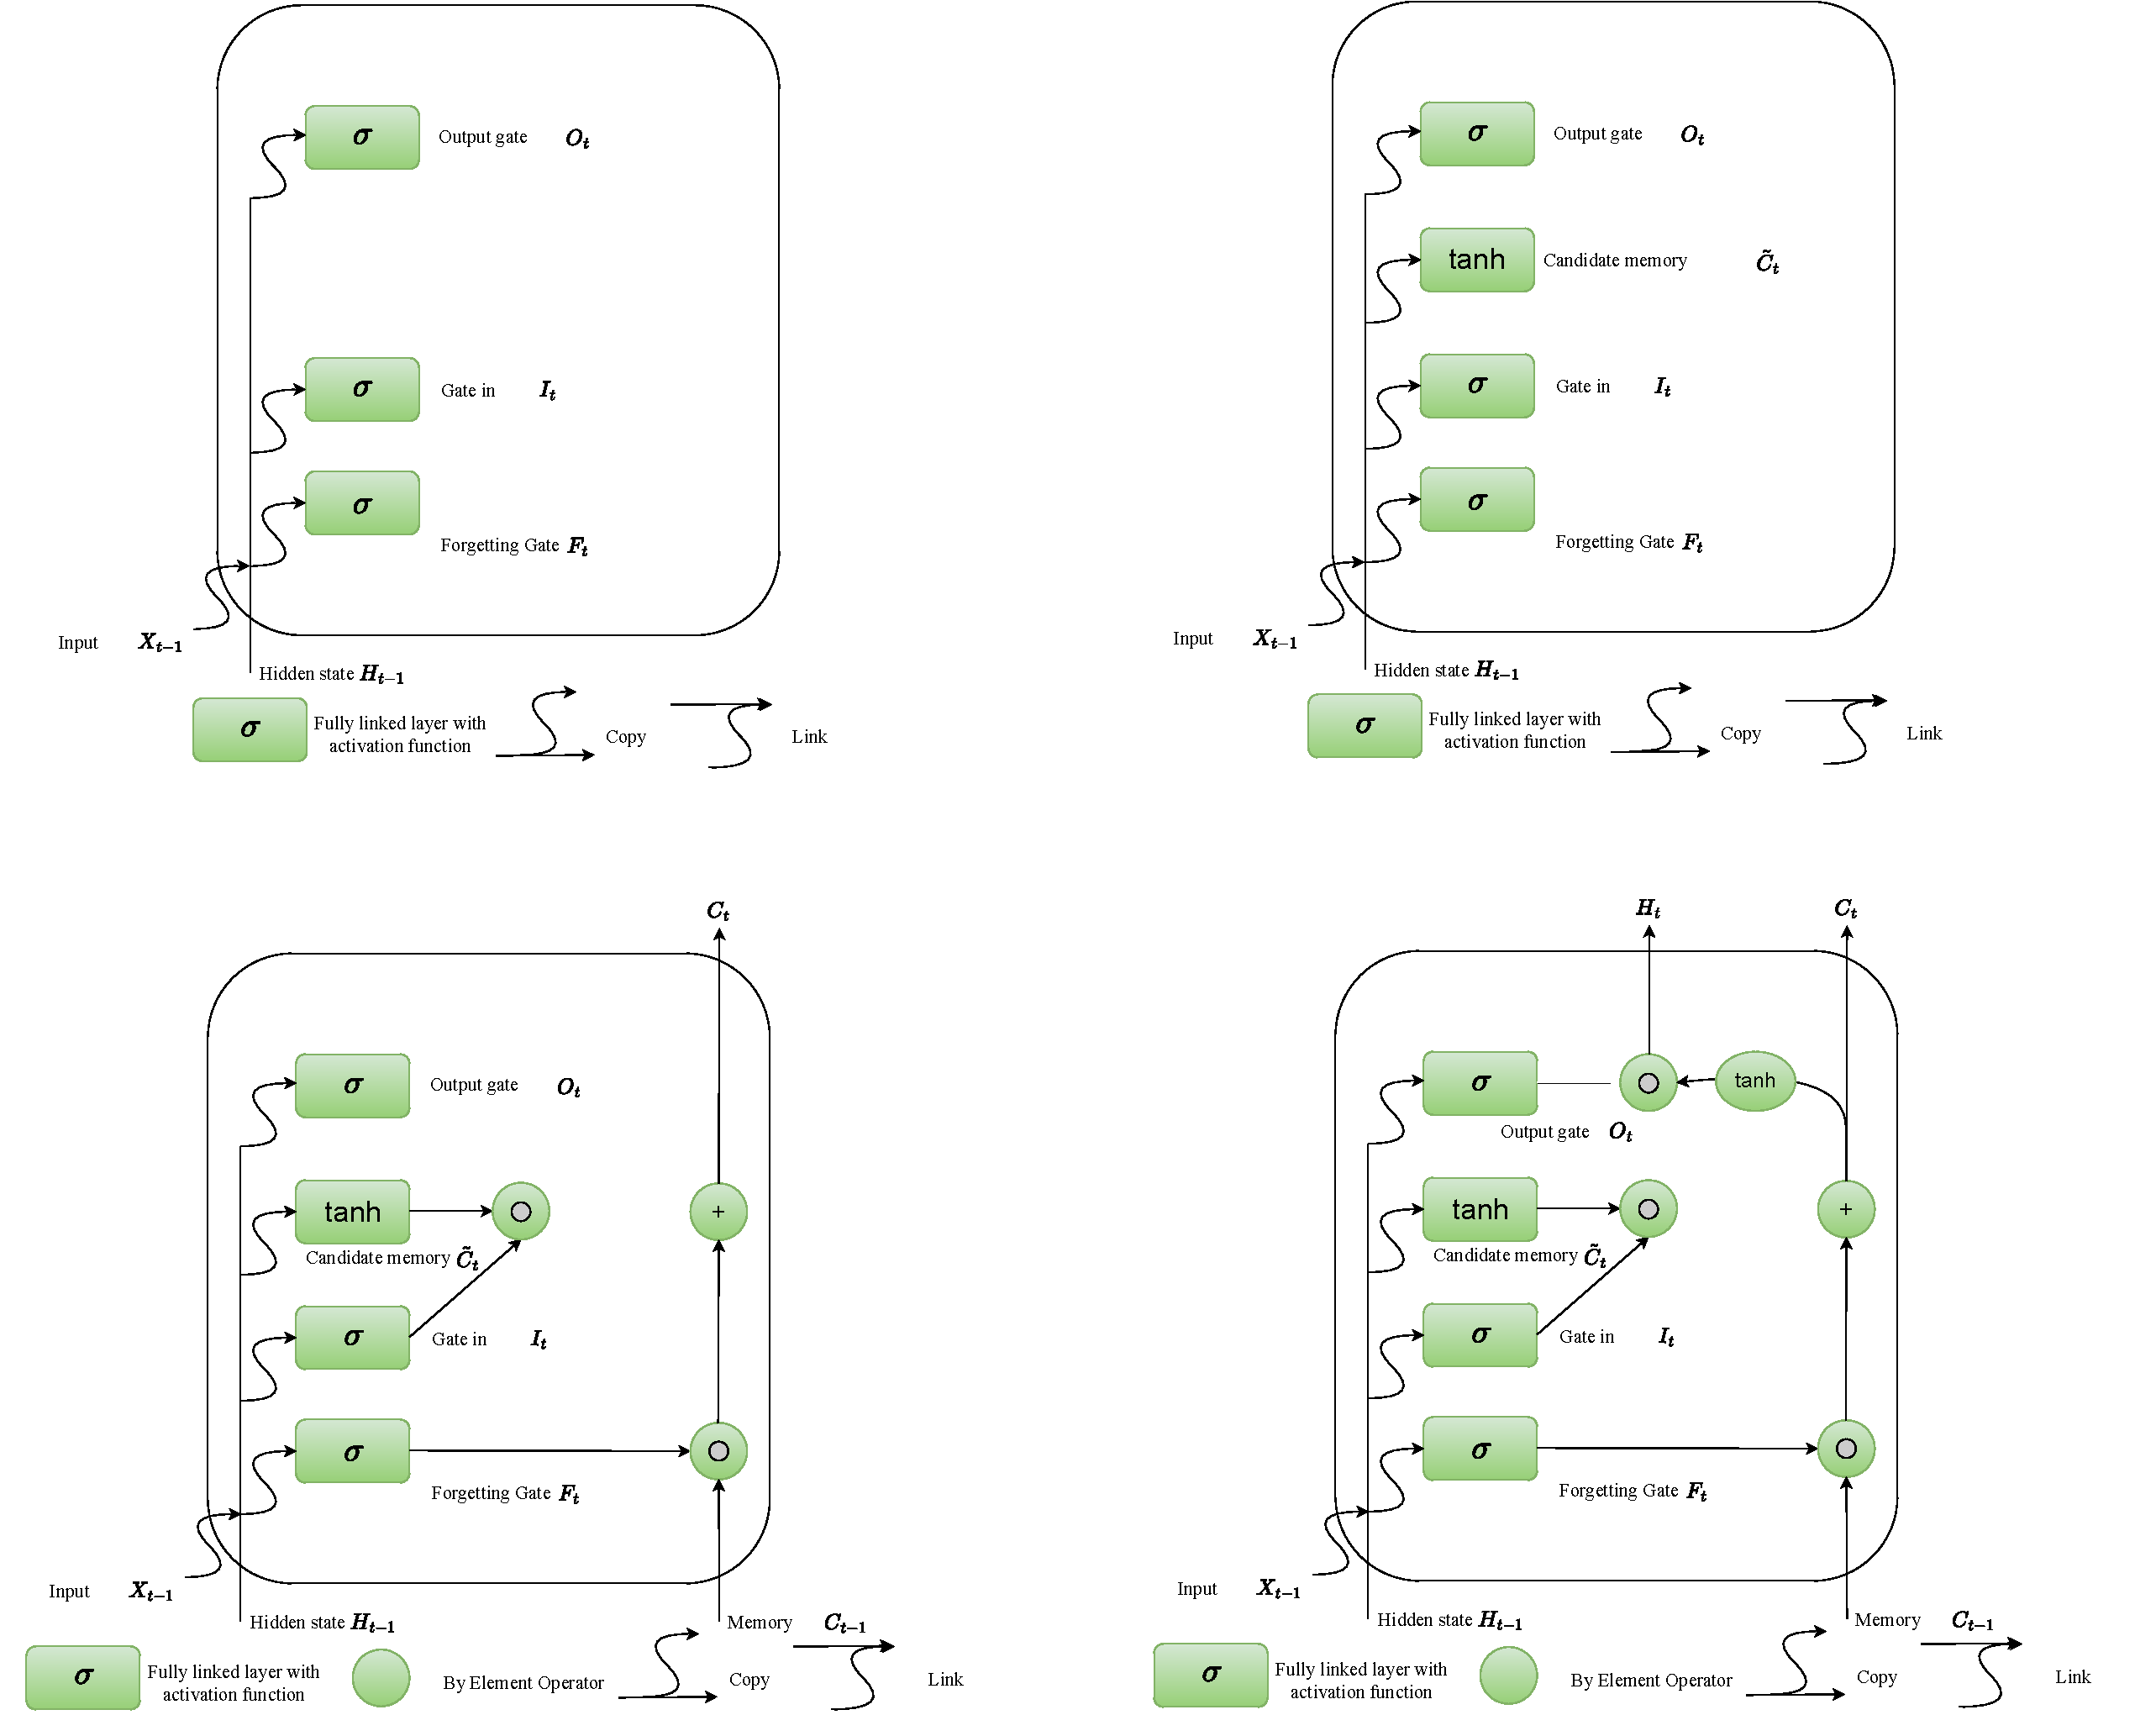
\includegraphics[width=0.75\textwidth]{picture/lstm.pdf} 	% 图片相对位置
    \caption{LSTM operating diagram}		% 图片标题 
    \label{fig:5655}							% 图片标签
\end{figure}
\FloatBarrier

As previously mentioned, the forget gate is represented by \(f_t\), which determines how much data from the prior internal state must be forgotten, and the input gate is represented by \(i_t\), which determines how much data must be saved from the current candidate state. An output gate called \(o_t\) regulates the amount of data that must be output from the internal state that is currently in the external state following nonlinear activation. The following is its formula:

\begin{equation}
	\begin{cases}
		f_t = \sigma(W_f^tx_t + U_f^Th_{t-1}+b_f)\\[3pt]
		i_t = \sigma(W_i^tx_t + U_i^Th_{t-1}+b_i)\\[3pt]
		o_t = \sigma(W_o^tx_t + U_o^Th_{t-1}+b_o)
	\end{cases}
\end{equation}

The input is denoted by \(x_t \in \mathbb{R}^{n \times d}\) in the formulas, and the hidden state from the previous time step is represented by \(h_{(t-1)} \in \mathbb{R}^{n \times d}\). The bias terms for the forget gate, input gate, and output gate are \(b_f\), \(b_i\), and \(b_o\), respectively, whereas the weights for the forget gate, input gate, and output gate are \(W_f^t\), \(W_i^t\), \(W_o^t\).

The formula for calculating candidate memory cells is similar to the gates described earlier (input gate, forget gate, and output gate), but it uses the tanh function as the activation function. the output of the tanh function has an output range of \((-1, 1)\), which helps to keep the memory cell values within a reasonable range and thus avoids the problem of vanishing gradients or gradient explosion. The following is the formula for calculating a candidate storage unit for the time step \(t\):

\begin{equation}
	\tilde{C}_t = \tanh(X_t W_{xc} + H_{t-1} W_{hc} + b_c)
\end{equation}

In this equation, the candidate memory cell at time step \(t\) is represented by \(C_t\) in this equation, the input for the current time step is \(X_t\), the hidden state from the previous time step is \(H_{t-1}\), the weight matrix from the inputs to the candidate memory cells is \(W_{xc}\), and the weight matrix from the hidden state to the candidate memory cells matrix is \(W_{hc}\). The hyperbolic tangent activation function tanh transfers the weighted inputs to a range of values of \((-1, 1)\), and \(b_c\) is the bias term of the candidate memory cell.

Based on the previously constructed formula for evaluating the athlete's momentum, we calculate the athlete's momentum value at each moment and construct an LSTM neural network with this label.



\begin{figure}[htbp]
    \centering
    \includegraphics[width=0.75\textwidth]{picture/lstm四线图.pdf} 	% 图片相对位置
    \caption{LSTM operating diagram}		% 图片标题 
    \label{fig:sensitive_analysis1}							% 图片标签
\end{figure}
\FloatBarrier
After 100 rounds of training, the model achieved an accuracy of 81.32\% and the loss was reduced to 0.07. The learning curves shown in Fig. 2 indicate that the loss for both training and validation decreased overall over time and that the accuracy of the validation set was similar to that of the training set, which suggests that the model is not overfitting. The LSTM was successful in predicting the athlete's momentum at every instant in time, as seen by the comparison curve between the observed and predicted values of the athlete's momentum in the following figure.

We plot the winning probability curves for both athletes, as shown in Figure 15. It can be observed that the intersection points of the curves serve as turning points in the match.

\begin{figure}[htbp]
    \centering
    \includegraphics[width=0.75\textwidth]{picture/win_rate_plot_no_title.pdf} 	% 图片相对位置
    \caption{Player win rate curve}		% 图片标题 
    \label{fig:sensitive_analysis1}							% 图片标签
\end{figure}
\FloatBarrier

\subsection{Recommendations for Player Performance}
% \subsubsection{Selection of the Best Strategy}

First, we simplify the model by defining that each athlete has a series of actions, each with a corresponding winning probability:

\begin{equation}
	\begin{cases}
		S = \{s_1, s_2, \cdots, s_n\}\\[3pt]
		P = \{p_1, p_2, \cdots, p_n\}
	\end{cases}
\end{equation}

The winning probabilities corresponding to each of these actions can be derived from the momentum statistics mentioned previously. When an opponent hits a ball in a certain way, their probability of winning is \(p_1\) and the probability of winning our counter action is \(p_2\). Then the probability of winning this action exceeds some threshold \(\varepsilon\):

\begin{equation}
	\begin{cases}
		p = p_2 \times (1 - p_1)\\[3pt]
		p > \varepsilon
	\end{cases}
\end{equation}

At this point, the corresponding \(p_2\) is:

\begin{equation}
	p_2 > \dfrac{\varepsilon}{1 - p_1}
\end{equation}

Therefore, actions with a probability of winning greater than \(p_2\) should be selected from the sequence of actions in the counterattack.

For example, the depth of the second serves of Carlos Alcaraz and Novak Djokovic in a match is shown below:

\begin{figure}[htbp]
    \centering
    \includegraphics[width=0.75\textwidth]{picture/柱状图.pdf} 	% 图片相对位置
    \caption{Player win rate curve}		% 图片标题 
    \label{fig:11}							% 图片标签
\end{figure}
\FloatBarrier

When we set the threshold to \(\varepsilon = 0.8\), assuming that Carlos Alcaraz has a higher probability of having a shallow depth of serve on his second serves, then Novak Djokovic should consider shifting his position back a little to improve the quality of his returns.

\subsection{Some recommendations for players}

\begin{itemize}
	\item \textbf{Opponent}
	\begin{enumerate}[label=\alph*.]
		\item \textbf{Data Analysis}
		
        It is important to thoroughly analyse your opponent before a match. Use historical video data and other resources to gain insight into your opponent's performance and win percentages in past matches. Analyse how your opponent reacts in a given situation.		
        \item \textbf{Simulation Training}
		
		Based on the opponent's data characteristics, conduct pre-match simulations and formulate tactics in advance.
	\end{enumerate}
	\item \textbf{Player's Self}
	\begin{enumerate}[label=\alph*.]
		\item \textbf{Data Analysis}
		
		It is essential to know yourself thoroughly before a match. Identify the situations you excel in and your winning percentage, analyse your moments of high or low momentum and work on strengthening your weaknesses.	
		\item \textbf{Psychological Factors}
		
		Mental factors are often the most influential factors on the outcome of a game, apart from an athlete's physical ability. Good athletes have good psychological qualities, which enable them to remain calm under pressure and turn pressure into motivation, thus achieving excellent results.
	\end{enumerate}
	\item \textbf{On-site Factors}
	\begin{enumerate}[label=\alph*.]
		\item \textbf{Strategic Adjustments}

        During a match, players should have a strong grasp of the situation on the field and know exactly when they have the upper hand and when they are at a disadvantage. Athletes need to adjust their mindset and strategy in a timely manner, accurately manage their physical condition and adopt different strategies at different stages of the game.
		
		\item \textbf{Coaching Factors}
		
		Athletes should communicate with their coaches during breaks. Coaches should use the model to analyse the game, provide key guidance to athletes during short breaks, address technical issues and point out weaknesses in their opponents. At the same time, coaches should also aim to stimulate momentum in their athletes to improve their performance.
	\end{enumerate}
\end{itemize}

\section{Momentum Index Modelling on Other Races}

The Heat and Celtics meet again in the 2023 NBA Eastern Conference Finals in a best-of-seven series. Butler's three-point shutout fell short, but he vowed to come back for the kill in the same situation. However, this time the Heat beat the Celtics 103-84 on the road to eliminate their rivals 4-3 and advance to the Finals, where they will face the Denver Nuggets.

\begin{figure}[htbp]
    \centering
    \begin{minipage}{0.45\textwidth} % 左侧部分
        \centering
        \includegraphics[width=\textwidth]{picture/第四问饼状图.pdf} % 替换为你的图片文件名
        \caption{Pie Chart of Data Sources} % 图片标题
        \label{fig:example_image} % 图片标签,用于引用
    \end{minipage}\hfill % hfill 用于两个 minipage 之间添加一些水平空间
    \begin{minipage}{0.55\textwidth} % 右侧部分
        \centering
        \captionof{table}{Website of Data Source} % 表格标题
        \label{tab:your_label_here} % 表格标签,用于引用
        \begin{tabular}{c} % 表格内容开始
            \toprule
            Database Websites \\
            \midrule
            \url{https://www.youtube.com}              \\
            \url{https://www.bleacherreport.com}       \\
            \url{https://www.espn.nl}                  \\
            \url{https://www.basketball-reference.com} \\
            \url{https://global.nba.com/scores/#!/}    \\ \hline

            \bottomrule
        \end{tabular}
    \end{minipage}
\end{figure}

During the game, both teams shot a low percentage from the field, with the Heat hitting only two shots halfway through the first quarter and the Celtics missing all of their first 12 threes. This led to a low momentum index graph at the beginning of the game with small swings for both teams. However, the Heat's Momentum Index gradually grew.

Mazzulla pep-talked his team before the game, stating that the game might be long, but the players should enjoy it. However, the Celtics were slow to find their form in the steal. In the first quarter, the Heat took the initiative to call a timeout when they were ahead, only to be overtaken by the Heat's 11-2 offensive wave.

The Celtics scored a total of five points on 2-of-15 shooting in the second seven minutes of the first quarter, leading to a 22-15 lead for the Heat at the end of the first quarter, the same as the Celtics' lowest scoring first quarter of the season. The Celtics' sluggish offence did not improve in the second quarter, as the Heat started the second quarter with a Robinson three-pointer and a Hay-Smith steal of Tatum with an assist to Vincent for a layup, leading to the Heat calling another game. The Heat extended their deficit to as many as 18 points during the second quarter. Though the Celtics were able to chase down consecutive points, led by Tatum, they still trailed the Heat 41-52 at halftime. This is consistent with the Momentum Chart performance, where the Heat led in scoring throughout the first half, and both teams' Momentum Indexes were on the rise. Additionally, the Celtics struggled from three-point range in the first half, hitting only four of their 21 attempts for a 19\% clip.

It's worth noting that on the Celtics' only off day, when they were down 0-3, Horford suggested that Mazzulla forgo the video lessons and gather the team to play golf to relax. Gervais recalled the occasion this way: "We skipped the video session altogether, we got away from basketball and focused on each other, trying to get our camaraderie back. We kind of lost touch under the pressure, but we were able to enjoy time with each other again."

As it happens, the module of game pressure is also considered in our momentum index model, and at one point in the post-break day game, the Celtics overtook the Heat in the momentum index, and since then, the Celtics have pulled out three straight games Obviously, it's obvious that for the Celtics, it's how to handle the pressure that's the team's obsession.

When the Celtics will be close to the score, this section, Martin hit a number of difficult shots, a single section of 4 shots to get 9 points, the end of the three sections of 14 shots 10 contributed 23 points and 8 rebounds. Greatly encouraging the morale, the Heat's momentum once again achieved rapid growth, successfully overtook the Celtics. In the subsequent fourth quarter, the Heat continued to team bloom, once the difference will be opened to more than 20 points, the NBA East final this suspense end.

After collecting various data about this game, we substituted them to calculate the momentum of both teams and plotted the momentum index curve against the total goals scored in this game as shown below:

\begin{figure}[htbp]
    \centering    
    \subfigure[]{				% 图片1([]内为子图标题)
    \label{Fig.sub.Flexibility_33.70}							% 子图1的标签
    \includegraphics[width=0.51\textwidth]{picture/第四问的动量图.pdf}}			  % 子图1的相对位置
    \subfigure[]{				% 图片2
    \label{Fig.sub.Flexibility_26.66}						% 子图2的标签
    \includegraphics[width=0.42\textwidth]{picture/第四问的比分变化图.pdf}}
    \caption{Momentum Index and Section Score Data for Two Teams}		% 总图标题
    \label{Fig:Flexibility}									% 总图标签
\end{figure}

The two curves matched by 65.918\%.

\section{Sensitive analysis}

The sensitivity of the model is crucial to its stability, and it is related to whether the model will be disturbed by some other factors. In order to test the sensitivity of the model, we increased and decreased speed\_mph by 0.5\% respectively, and then input it into lstm to observe the change of accuracy when lstm predicts. The prediction results for these three cases are shown below:

\begin{figure}[htbp]
    \centering
    \includegraphics[width=0.75\textwidth]{picture/灵敏度.pdf} 	% 图片相对位置
    \caption{Sensitivity test curve}		% 图片标题 
    \label{fig:sensitive_analysis1}							% 图片标签
\end{figure}
\FloatBarrier

As can be seen from the figure, when increasing or decreasing the speed\_mph by 0.5\% for speed\_mph, the trend of the accuracy level does not change and stays within the acceptable range. Therefore, we can conclude that our model is stable and capable of solving practical problems.

\section{Strengths and Weaknesses}
\subsection{Strengths}
\begin{itemize}
    \item Our model provides a more objective and comprehensive quantitative portrayal of player momentum, with G1-entropy weights-independence weights integrating the subjective and objective aspects of momentum, and this approach is not only applicable to tennis, but also relevant to the game in general.
    \item The DTW model reasonably demonstrates that momentum exists and more accurately compares the correlation between momentum and fluctuations in athlete levels.
    \item The lstm model can predict complex nonlinear problems and addresses the shortcomings of the traditional ARIMA model.
\end{itemize}
\subsection{Weaknesses}
\begin{itemize}
    \item The predictions of the model are based on the metrics of the given dataset, but the presence of metrics that influence the predictions but are not in the dataset may result in a less accurate model.
    \item The lstm model requires a large dataset, however limited data can lead to model overfitting.
\end{itemize}

\section{Conclusion}
In summary, this paper firstly establishes a G1-entropy weight-independence weight evaluation model, which comprehensively evaluates the momentum from subjective and objective aspects respectively. We determined the weights of each index, and made a quantitative mathematical assessment of the player's momentum.

We then used the DTW model to determine the similarity between the momentum curve and the player's score curve, thus proving that momentum exists, and showing that there is indeed a momentum factor that determines the movement of the outcome of a tennis match.

Then, we used ARIMA model to predict the momentum of the athlete, and found that its matching degree was not very accurate, we analysed that this might be related to the fact that ARIMA is good at predicting the linear part. So we used the lstm model to predict the momentum of this complex non-linear problem, and found that the results are better. We defined the winning percentage with the help of momentum, made a winning percentage graph and found that the intersection of the winning percentage curves of two athletes is the turn of the match. We have analysed the game briefly using game theory and have given some suggestions to the athletes.

Finally, a sensitivity analysis of the lstm model was done and it was found that when increasing or decreasing the speed\_mph by 0.5\% for the speed\_mph, the accuracy of the model varied within acceptable limits.

\section{The future and outlook of modelling}

Our momentum index model has done an excellent job in that problem, being able to correctly determine how high or low a player's momentum is during a match, and thus how well the player is performing. However, since there is more to actual matches than just the data provided, the model is not accurate enough and does not generalise well enough in new tennis tournaments as well as other tournaments, which is an obvious problem.

Therefore, we have the following outlook on the model and anticipate that it will be updated and further refined in the future in order to increase the model's accuracy and generalizability. Firstly, the sample categories of the dataset should be richer, and factors such as weather and players' head-to-head record should be included. Secondly, the number of data samples should be more huge, only when the number of samples goes up, the model is not easy to be overfitted and the generalisation can be improved. Then, our model is rough, and the matching degree only considers the DTW algorithm, which should be considered with more methods, or even a combination of different methods to make the results more accurate. Finally, our model lacks comparison, similar to logistic regression, random forests and other methods we have not modelled and calculated, resulting in a lack of side-by-side comparisons of our model, it is better, but not necessarily the best model.

Not only that, in model III, we also only consider ARIMA and LSTM two models, the use of models is not broad enough at the same time, but also shallow, if the other time series methods or ARIMA and LSTM for the integrated use of the model, perhaps the model will be more accurate, there will be better models and algorithms used in the LSTM.

In the limited time we had, we built an excellent model, but clearly not the best one. We hope that in the future we can improve our model by more efforts, and we also hope that our model can play an innovative role in solving this kind of problems and lay a solid foundation for future generations. We hope that our model has a bright future.

\newpage

\ThisCenterWallPaper{1}{poster.pdf}
\addcontentsline{toc}{section}{Memo}
\vspace*{0.5cm}

\newpage


% 参考文献,此处以 MLA 引用格式为例
\clearpage
\begin{spacing}{0.01}
\begin{thebibliography}{99}
    % \bibitem{1} Leighton, F. Thomson. \emph{Introduction to parallel algorithms and architectures: array, trees, hypercubes}. 2014.
    % \bibitem{2} Clemente, Filipe Manuel, et al. "General network analysis of national soccer teams in FIFA World Cup 2014." \emph{International Journal of Performance Analysis in Sport} 15.1 (2015): 80-96.
    % \bibitem{3} Dijkstra, Edsger Wybe. "A Note on Two Problems in Connexion With Graphs." \emph{Numerische Mathematik} 1(1959):269-271.
    % \bibitem{4} Ahnert, Sebastian E., et al. "Ensemble approach to the analysis of weighted networks.." \emph{Physical Review E} 76.1 (2007).
    % \bibitem{5} Wong, J. A. Hartiganm. A. . "Algorithm AS 136: A K-Means Clustering Algorithm." \emph{Journal of the Royal Statistical Society. Series C (Applied Statistics)} 28.1(1979):100-108.
    % \bibitem{6} Buldu, J. M., et al. "Defining a historic football team: Using Network Science to analyze Guardiola’s F.C. Barcelona." \emph{Scientific Reports} 9.1 (2019): 1-14.
    % \bibitem{7} \emph{Balotelli sends Italy past Germany}. (2012). Retrieved December 10, 2014, from\url{https://www.uefa.com/uefaeuro/season=2012/matches/round=15174/match=2003379/index.html}
    % \bibitem{8} Sigari, Mohamad Hoseyn, et al. "Counterattack detection in broadcast soccer videos using camera motion estimation." \emph{international symposium on artificial intelligence} (2015): 101-106.
    % \bibitem{9} Abdelmahmoud Hassan Elsheikh. \emph{Effect of Leadership Intensity on Integrating Some Formal and Informal Organizational Efforts for Community Development in Khartoum Province}. 2016.
    \bibitem{1} Hochreiter, S., \& Schmidhuber, J. (1997). Long short-term memory. *Neural Computation*, 9(8), 1735-1780. 
    \bibitem{2} Maalouf, M. (Year). Logistic regression in data analysis: An overview. Journal/Publisher.
    \bibitem{3} Author(s). (Year). Title of the article. Journal/Conference.
    \bibitem{4} \url{https://medium.com/draftkings-engineering/building-a-tennis-simulation-d6afdaa97d19}
    \bibitem{5} Pan, Ouyang, Wu, Ecaterina, Ion, Jiao et al. (Year). Title of the Article. *Frontiers in [specific field or journal section]*.
    \bibitem{6} Shannon, C.E. (1948). A Mathematical Theory of Communication. Bell System Technical Journal, 27(3), 379-423.
    \bibitem{7} Shannon, C.E. (1948). "A Mathematical Theory of Communication". *Bell System Technical Journal*, 27(3), 379-423, 623-656.
    \bibitem{8} Little, R.J.A., \& Rubin, D.B. (2014). This work is a foundational reference on missing data imputation.
    \bibitem{9} Han, J., Pei, J., \& Kamber, M. (2011). *Data Mining: Concepts and Techniques* (3rd ed.). Morgan Kaufmann.
    \bibitem{10} \url{https://www.infona.pl/resource/bwmeta1.element.ieee-art-000006115088}
    \bibitem{11} Zeleny, M. (1982). "Multiple Criteria Decision Making". *McGraw-Hill*.
    \bibitem{12} Li, X., \& Liu, L. (2015). "A novel method to determine the weights of indicators in a combined evaluation model based on entropy weight". *Journal of Computational and Applied Mathematics*, 277, 73-80.
    \bibitem{13} Wang, Z., \& Zeng, S. (2009). "A multi-criteria decision-making method based on a cross-entropy with interval numbers". *Knowledge-Based Systems*, 22(8), 586-589.
    \bibitem{14} Li, R., \& Li, D. (2005). The Empirical Research on the Comprehensive Evaluation of the Regional Economic Competitiveness Based on Entropy Method. Systems Engineering, 23(2), 22-26.
    \bibitem{15} Sakoe, H., \& Chiba, S. (1978). Dynamic programming algorithm optimization for spoken word recognition. *IEEE Transactions on Acoustics, Speech, and Signal Processing*, 26(1), 43-49. 
    \bibitem{16} Berndt, D. J., \& Clifford, J. (1994). Using dynamic time warping to find patterns in time series. In *Proceedings of the 3rd International Conference on Knowledge Discovery and Data Mining (KDD-94)* (pp. 359-370).
    \bibitem{17} Keogh, E., \& Ratanamahatana, C. A. (2005). Exact indexing of dynamic time warping. *Knowledge and Information Systems*, 7(3), 358-386.
    \bibitem{18} Box, G.E.P., \& Jenkins, G.M. (1970). *Time Series Analysis: Forecasting and Control*. San Francisco: Holden-Day.
    \bibitem{19} Graves, A. (2012). Supervised sequence labelling with recurrent neural networks. In *Studies in Computational Intelligence* (Vol. 385). Springer, Berlin, Heidelberg.
    \bibitem{20} Gers, F. A., Schmidhuber, J., \& Cummins, F. (2000). Learning to forget: Continual prediction with LSTM. *Neural Computation*, 12(10), 2451-2471.

\end{thebibliography}
\end{spacing}

\newpage

\clearpage
\begin{spacing}{1.2}
    \begin{center}
        {\LARGE \uline{Report on Use of AI}} % 设置标题,使用 \uline 为标题加下划线
        % \addcontentsline{toc}{section}{Report on Use of AI}
    \end{center}

    \begin{enumerate}
        \item {
            Chatgpt 4.0
            \begin{tcolorbox}[colback=gray!20, boxrule=0pt] % 设置背景色为浅灰色,这里 20 表示颜色的深浅程度
            \textbf{Query1:} Can DTW algorithm be used to calculate curve matching degree?
            \end{tcolorbox}
            \begin{tcolorbox}[colback=gray!5, boxrule=0pt]
            \textbf{Output:} Yes, the Dynamic Time Warping (DTW) algorithm can be used to compute the similarity between curves, effectively measuring the degree of match between them. DTW is a powerful technique that allows for the comparison of two temporal sequences which may vary in time or speed. In the context of curve matching, DTW can align points on two curves in a way that minimizes the overall distance between them, taking into account the temporal distortion between the curves. This makes DTW particularly useful in applications where the shapes of the curves are similar but they are not perfectly aligned in the time axis, such as in time series analysis, speech recognition, and in the analysis of any data that can be represented as a curve or a sequence over time.
            \end{tcolorbox}
        }

        \item {
            Chatgpt 4.0
                \begin{tcolorbox}[colback=gray!20, boxrule=0pt] % 设置背景色为浅灰色,这里 20 表示颜色的深浅程度
                \textbf{Query2:} What are the basic steps of DTW?
                \end{tcolorbox}

                \begin{tcolorbox}[colback=gray!5, boxrule=0pt]
                \textbf{Output:} The basic steps of Dynamic Time Warping (DTW) include: 
                    \begin{itemize}
                        \item creating a cost matrix to store distances between elements of two time series, 
                        \item using dynamic programming to fill this matrix with the aim of finding the minimum cumulative distance, and 
                        \item tracing back from the bottom right corner of the matrix to find the optimal path that aligns the two series. This process allows for the comparison of two sequences that may vary in time, by optimally aligning them despite their differences in speed or timing.
                    \end{itemize}
                \end{tcolorbox}
        }

        \item {
            Chatgpt 4.0
            \begin{tcolorbox}[colback=gray!20, boxrule=0pt] % 设置背景色为浅灰色,这里 20 表示颜色的深浅程度
            \textbf{Query3:} Whether LSTM can be used for time series prediction?
            \end{tcolorbox}
            \begin{tcolorbox}[colback=gray!5, boxrule=0pt]
            \textbf{Output:} Yes, Long Short-Term Memory (LSTM) is a type of deep learning model that is suitable for time series prediction. LSTMs are a variant of recurrent neural networks (RNNs) designed to handle and learn long-term dependencies in time series data.
            
            Time series data exhibits temporal patterns with data points changing over time. LSTM models, with their internal memory units, can capture and learn long-term dependencies in sequences, making them well-suited for time series prediction tasks.
            \end{tcolorbox}

            \begin{tcolorbox}[colback=gray!5, boxrule=0pt]
            When using LSTM for time series prediction, it is common to split the data into training and testing sets. The model is trained on the training set, and then its performance is evaluated on the testing set. The model takes past time steps as input and predicts future time steps.
            
            In summary, LSTM is a powerful tool for time series prediction, but careful tuning of model parameters, selection of appropriate features and data preprocessing methods, and thorough model evaluation and optimization are essential for achieving optimal performance in specific applications.
            \end{tcolorbox}

        }

        \item {
            Chatgpt 4.0
            \begin{tcolorbox}[colback=gray!20, boxrule=0pt] % 设置背景色为浅灰色,这里 20 表示颜色的深浅程度
            \textbf{Query4:} What are the disadvantages of LSTM?
            \end{tcolorbox}
            \begin{tcolorbox}[colback=gray!5, boxrule=0pt]
            \textbf{Output:} While LSTM is a powerful deep learning model, it does have some drawbacks, including:

            \begin{itemize}
                \item High Computational Cost: LSTM models often require significant computational resources, especially when dealing with large datasets or complex model structures. This can result in long training times and a need for powerful hardware.
                
                \item Complex Hyperparameter Tuning: LSTMs have many hyperparameters to tune, such as learning rate, the number of layers, and the number of hidden units. Choosing appropriate hyperparameters may require extensive experimentation and experience.
                
                \item Risk of Overfitting: On small datasets or without proper regularization techniques, LSTMs may be prone to overfitting, leading to poor performance on unseen data.
                
                \item Difficult to Explain: Deep learning models, including LSTMs, are often considered black-box models. Explaining the decision-making process and how specific patterns are learned can be challenging.
                
                \item Vanishing and Exploding Gradients: Despite being designed to address the vanishing gradient problem, LSTMs may still encounter issues of vanishing or exploding gradients in certain situations, affecting training stability.
                
                \item Data Intensity: For more complex tasks, LSTMs typically require a large amount of training data to fully leverage their advantages. In situations with scarce data, overfitting or insufficient learning of complex patterns may occur.
            \end{itemize}
            
            Despite these drawbacks, LSTM remains a preferred model for many time series and sequence modeling tasks. However, its advantages and limitations should be carefully considered and balanced based on specific application requirements.
            \end{tcolorbox}
        }

    \end{enumerate}
\end{spacing}
\end{document}  % 结束